\documentclass[a4paper,12pt]{article}
\usepackage[utf8]{inputenc}
\usepackage[english]{babel}
\usepackage{authblk}
\usepackage{graphicx}
\usepackage{mathptmx}
\usepackage[singlespacing]{setspace}
\usepackage[headheight=1in,margin=1in]{geometry}
\usepackage{fancyhdr}
\usepackage{comment}
\usepackage{wrapfig}
\usepackage[font=footnotesize]{caption}

\usepackage{amsfonts}
\usepackage{amsmath}
\usepackage{csquotes}
\usepackage{wrapfig}
\usepackage{subcaption}
\usepackage[colorlinks=true,linkcolor=blue,citecolor=blue,urlcolor=blue]{hyperref}

\renewcommand{\headrulewidth}{0pt}
\pagestyle{fancy}

\chead{
$4^{th}$ International Conference on the Science of Science \& Innovation\\June 29 -- July 1, 2026, University of Colorado Boulder, Boulder, CO, USA}


\title{\vspace{-2.5em}Who funds Open Science? : A dashboard to track data sharing in publications across major funders}

\author[1]{Josh Lawrimore}
\author[2]{Christoph Li}
\author[2]{Dustin Moraczewski}
\author[2]{Adam Thomas}

\affil[1]{Clinical Monitoring Research Program Directorate, Frederick National Laboratory for Cancer Research}
\affil[2]{Data Science \& Sharing Team, National Institute of Mental Health}

\date{}

\begin{document}

\vspace{-2em}
\maketitle
\thispagestyle{fancy}

\vspace{-2em}
\noindent\textit{Keywords: open data, science policy, research transparency}

\section*{Extended Abstract}

Open data sharing is central to the reproducibility and transparency of scientific research~\cite{Wilkinson2016, Baker2016}. Major funders have adopted data sharing mandates of varying design---the U.S.\ National Institutes of Health implemented its latest Data Management and Sharing Policy in January 2023~\cite{NIH2023dms}, while the Wellcome Trust and European Research Council have maintained similar requirements since 2017. Journals have also strengthened data availability requirements. Yet whether these policy instruments produce measurable differences in rates of compliance in the published literature remains difficult to quantify at scale. In an analysis of 2.75 million articles from the PubMed Central Open Access Collection (PMC OA), Serghiou et al.~\cite{Serghiou2021-pl} showed that by 2020 data sharing rates had reached only ${\sim}$15\%. Since then, tools for accurate detection of data availability statements have dramatically improved and limitations of open access XML---including omission of data availability statements---have been recognized. The current project aims to provide interactive, accurate measurement of data sharing to evaluate which funders and policy designs are most effective---a core question for the science of science.

We analyzed approximately 784,000 open access biomedical research articles published between January 2024 and June 2025. Full-text was extracted from approximately 257,000 PDFs using MinerU~\cite{Wang2024mineru}, a machine learning-based document extraction tool, and analyzed with oddpub v7.2.3~\cite{Riedel2020}, which detects open data and open code sharing statements through pattern matching. Article-level metadata---including funder, journal, and institutional affiliations---was obtained from OpenAlex~\cite{Priem2022}. Funder names were normalized across 816 funders. For the remaining ~527,000 articles with only XML coverage, we applied journal-specific correction factors derived from head-to-head PDF versus XML comparisons, reporting 95\% Wilson score confidence intervals on corrected estimates.

We found an overall open data rate of 8.7\%, rising to 16.6\% among articles with identified funders. Rates varied substantially across major funders---defined as those exceeding a Weibull-derived article-count threshold and 100,000 aggregated OpenAlex works (Figure~\ref{fig:funders}). The Agence Nationale de la Recherche led at 26.1\%, followed by the U.S.\ National Science Foundation (24.7\%), the Wellcome Trust (24.1\%), the Swiss National Science Foundation (23.4\%), and the Deutsche Forschungsgemeinschaft (21.6\%). The NIH---the largest funder in the dataset with nearly 29,000 articles---achieved 20.5\%. After applying correction factors for XML-only coverage, estimated rates were higher across all funders (e.g., ANR 28.8\%, NSF 27.8\%). Several smaller funders with narrower portfolios achieved even higher observed rates and are available for exploration on the dashboard. Among journals, variation was even greater: genomics titles led---Nature Structural \& Molecular Biology (86.1\%), Microbial Genomics (84.8\%), Cell Genomics (80.2\%)---with corrected estimates reaching 92.9\% for Nature Genetics. PDF-based detection identified approximately 52\% more sharing statements than XML-based methods on the same articles.

\begin{figure}[h]
\centering
\vspace{-0.5em}
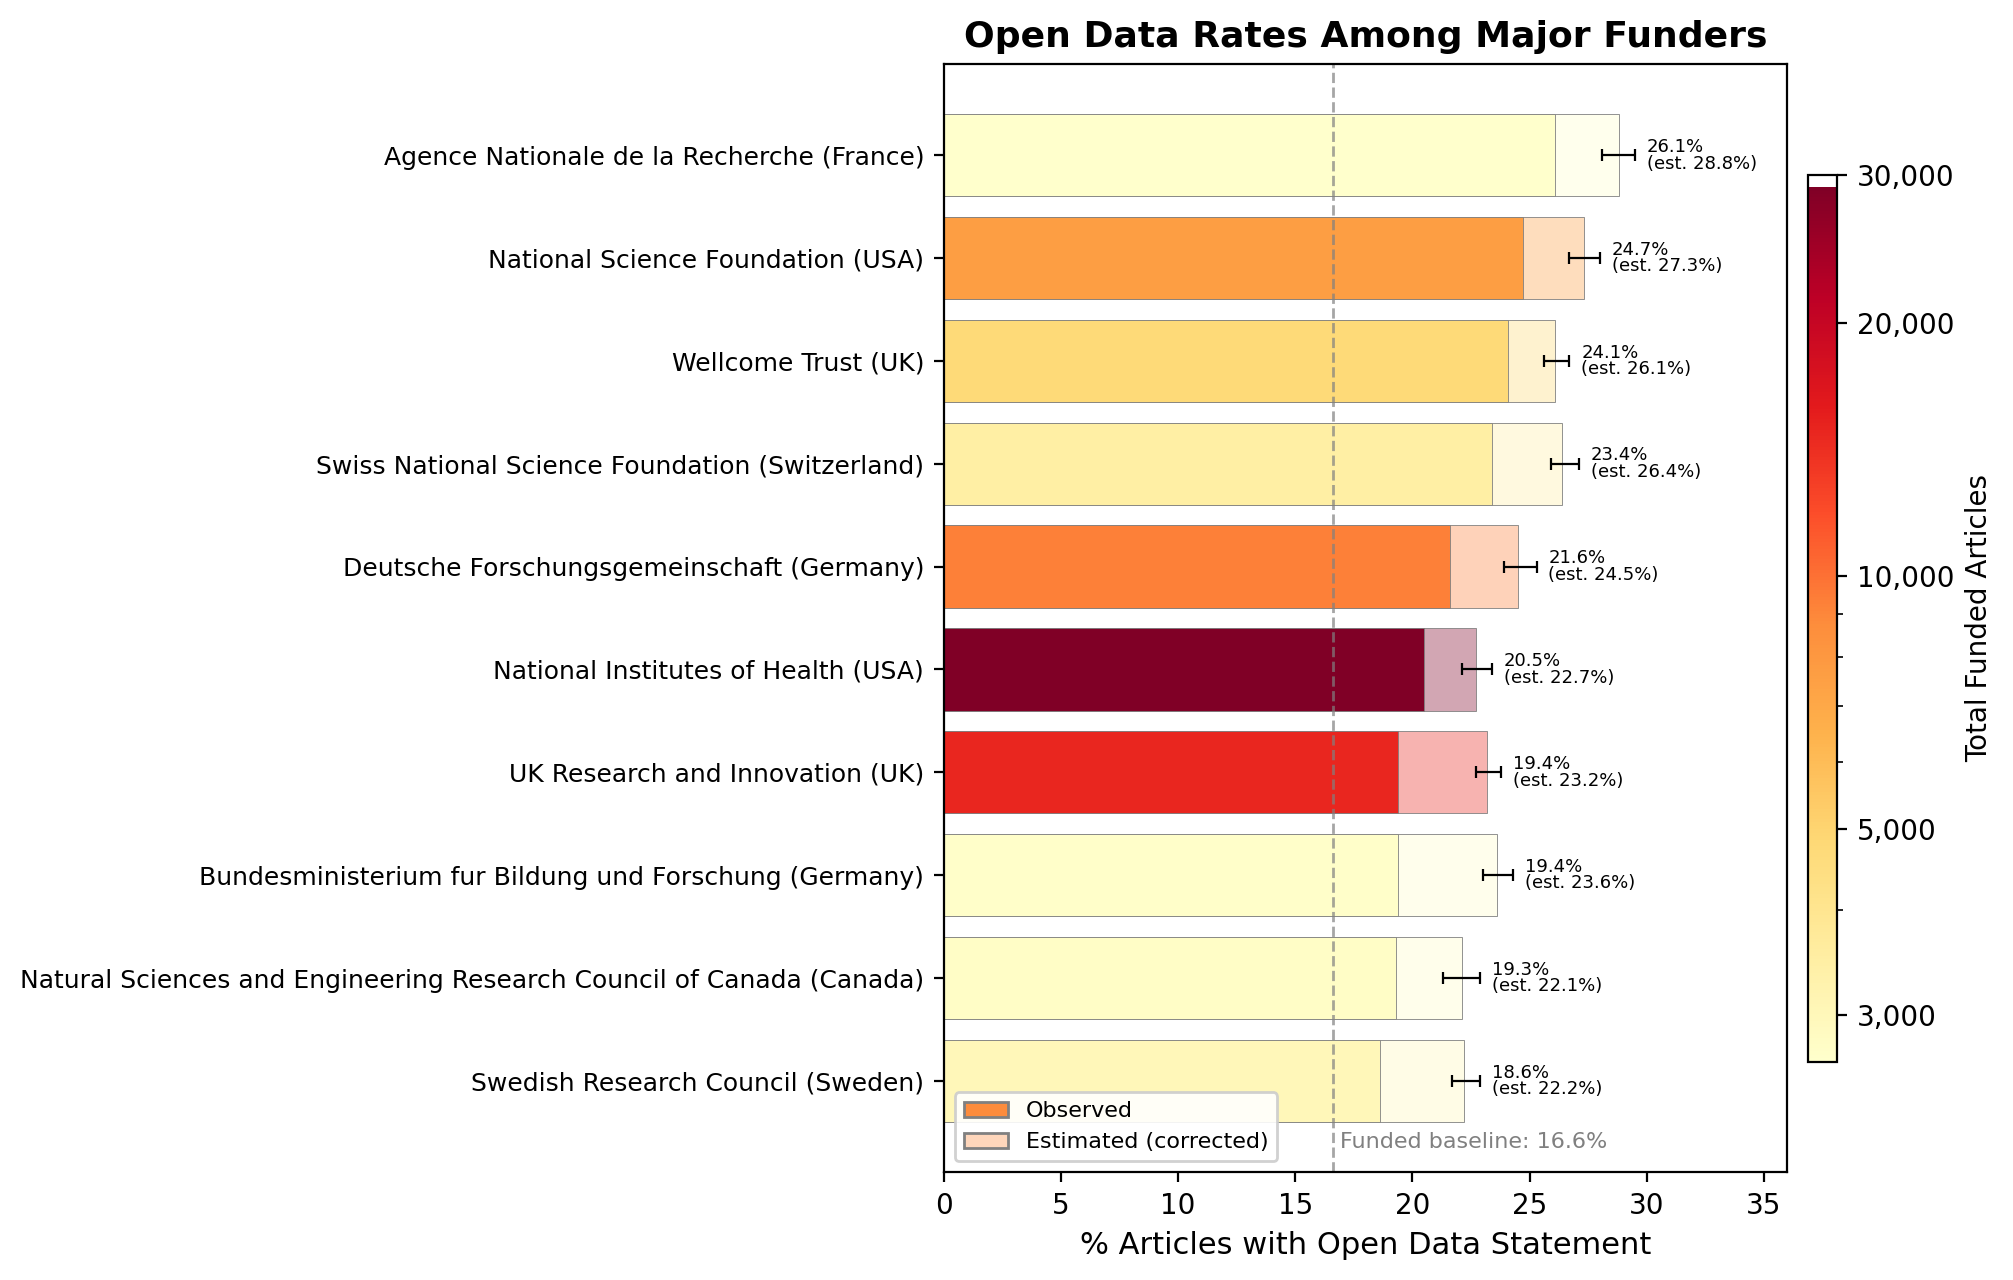
\includegraphics[width=0.82\textwidth]{funders_top10.png}
\caption{Open data rates among major biomedical funders (2024--2025). Bars show observed (solid) and corrected (light) rates; error bars are 95\% Wilson CIs. Color encodes article count (log scale). Dashed line: funded-article baseline (16.6\%).}
\label{fig:funders}
\vspace{-1em}
\end{figure}

This variation clusters by policy characteristics and disciplinary norms. Funders in data-intensive fields and those with strong cultures of openness achieve rates well above the baseline. Psychology journals form a distinct high-sharing cluster, reflecting norms that emerged after the replication crisis. These patterns indicate that policy specificity and enforcement---not merely the existence of a mandate---drive compliance. All results are explorable via an interactive dashboard at \url{https://www.opensciencemetrics.org}. Future work will expand the corpus and enable longitudinal analysis of policy changes such as the 2023 NIH Data Management and Sharing Policy.

\renewcommand{\refname}{\vspace{-0.5em}\normalsize References}
\renewcommand{\markboth}[2]{}
\begin{thebibliography}{9}\scriptsize\setlength{\itemsep}{1pt}\setlength{\parsep}{0pt}\setlength{\topsep}{0pt}
\bibitem{Wilkinson2016} Wilkinson et al., 2016. \textit{Sci.\ Data} 3:160018. \href{https://doi.org/10.1038/sdata.2016.18}{doi:10.1038/sdata.2016.18}
\bibitem{Baker2016} Baker, 2016. \textit{Nature} 533:452--454. \href{https://doi.org/10.1038/533452a}{doi:10.1038/533452a}
\bibitem{NIH2023dms} NIH, 2023. Final Policy for Data Management and Sharing. \href{https://sharing.nih.gov/data-management-and-sharing-policy}{sharing.nih.gov}
\bibitem{Serghiou2021-pl} Serghiou et al., 2021. \textit{PLoS Biol.}\ 19:e3001107. \href{https://doi.org/10.1371/journal.pbio.3001107}{doi:10.1371/journal.pbio.3001107}
\bibitem{Wang2024mineru} Wang et al., 2024. MinerU. \href{https://doi.org/10.48550/arXiv.2409.18839}{arXiv:2409.18839}
\bibitem{Riedel2020} Riedel et al., 2020. \textit{Data Sci.\ J.}\ 19:42. \href{https://doi.org/10.5334/dsj-2020-042}{doi:10.5334/dsj-2020-042}
\bibitem{Priem2022} Priem et al., 2022. OpenAlex. \href{https://doi.org/10.48550/arXiv.2205.01833}{arXiv:2205.01833}
\end{thebibliography}

\end{document}
